\chapter{Résumé détaillé}

\selectlanguage{french}

\section{Introduction : robots, interaction et connaissances}
\label{chapt|introduction}

Nao a été aperçu jouant avec des enfants autistes, Justin tapote sur la boite
de chocolat en poudre pour préparer le petit-déjeuner, des robots PR2 nous
amènent des bières et distribuent du popcorn dans les laboratoires, tandis que
Rosie s'occupe des crêpes pour le goûter : si ces expériences récentes, mises
en place un peu partout dans les laboratoires de robotique nous dise une chose,
c'est que la robotique de service est en train de quitter le domaine de la
science-fiction, des rêves, des fantasmes et s'apprête à frapper à la porte de
notre quotidien.

\begin{figure}[!h]
    \centering
    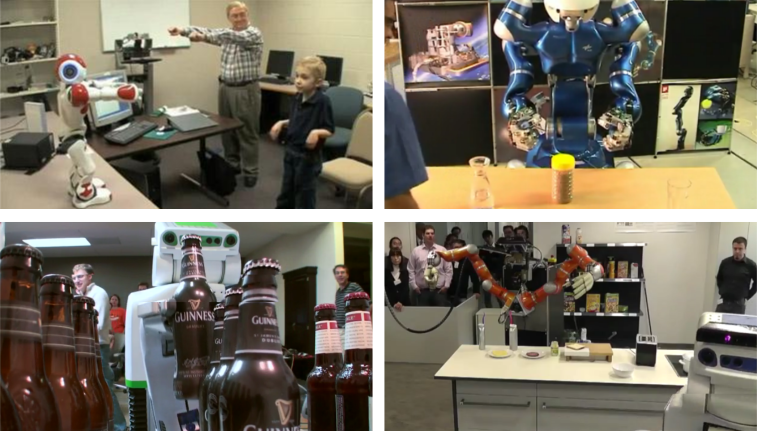
\includegraphics[width=0.8\columnwidth]{intro/everyday_robots.pdf}

    \caption*{Nao, Justin, PR2, Rosie: les robots jouent avec les enfants,
    préparent des chocolats chauds, décapsulent les bières et font sauter les
crêpes. Pour l'instant en laboratoire, sans interactions très avancées avec les
hommes. Que leur manquent-ils pour s'inviter dans nos maisons ?}

    \label{fig|everyday-robots}
\end{figure}

Des progrès considérables ont été accomplis au niveau de la perception des
robots : les caméras et les lasers sont aggrégés dans des pseudo-capteurs
renvoyant des informations de haut-niveau : reconnaissance de visages,
localisation et cartographie SLAM, posture dynamique des hommes... Permettre à
un robot de comprendre son environement est aujourd'hui un défi où deux
facettes se mèlent : reconstruire en continu un monde géométrique et dynamique
cohérent ; abstraire ce même monde en une représentation symbolique adaptée au
raisonnement logique.

La résolution de ce premier défi, auquel cette thèse tente de contribuer, n'est
cependant pas suffisante pour permettre une interaction entre hommes et robots.
Le robot auquel nous pensons vit dans le monde réel, un monde pour et avec des
humains. Notre robot doit acquérir des compétences sociales, il doit pouvoir
considérer les hommes autour de lui non seulment comme des entités physiques
(...sur lesquelles ils ne faut pas rouler par exemple), mais aussi et surtout
comme des entités intelligentes, dotées d'une individualité propre et unique.

Le robot doit pouvoir non seulement représenter son environement, représenter
son propre état mental, mais aussi tenter de deviner et de représenter l'état
mental, les connaissances des autres agents avec lesquels il interagit. Et ces
modèles, il faut ensuite savoir les mettre en \oe uvre pour donner corps  des
compétences sociales au premier rang desquelles se trouve la fonction de
communication.

\begin{figure}
    \centering
    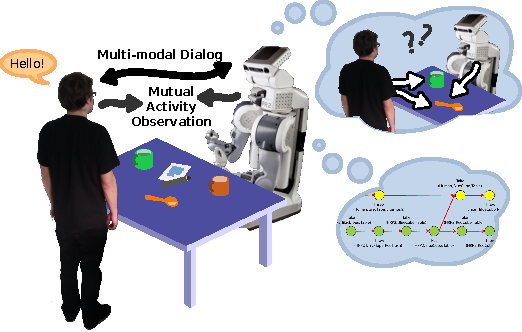
\includegraphics[width=0.9\columnwidth]{intro/grounding_robot.pdf}
    
    \caption{Le robot est plongé dans une \emph{situation}. Les source de
    connaissances sont multiples : dialogue multi-modal, observation de
    l'environement et des activités de l'homme, capacités internes de planification
    et de raisonnement symbolique. Le robot raisonne non seulement de son propre
    point de vue, mais en se projettant à la place des autres agents.}

    \label{fig|hri-dec}
\end{figure}

La figure~\ref{fig|hri-dec} résume les principaux aspects de l'interaction qui
nécessitent d'être traduit dans des modèles adaptés au robot. Du point de vue
du robot, plusieurs compétences cognitives sont impliquées : traitement du
dialogue (verbal et déictique : regard, posture, gestes...), acquisition et
maintient de un ou plusieurs modèles de l'environnement (non seulement du point
de vue du robot, mais aussi des points de vue de chacun des autres agents),
anticipation (quelles sont les intentions de l'humain ? Puis-je prédire ses
actions ?), planification et contrôle (comment puis-je progresser vers le but
?), suivi des activités des autres agents (est-ce que la coopération est
effective ?) et de l'avancement générale de la tâche.

Chacune de ces capacités cognitives se traduit en contraintes et besoins sur le
système de représentation de connaissances, comme nous allons le présenter
un peu après.



\subsection{Un programme}
\label{sect|challenges}

Cette brève introduction laisse deviner en négatif le programme de recherche que nous
défendons dans cette thèse, et que nous résumons ici. Nous pouvons essayer
d'articuler les trois défis liés au champ de la représentation des
connaissances dans la robotique de service et robotique-compagnon que nous
traitons dans ce travail de doctorat.

Notre premier objectif est en réalité de préciser cette notion de
\emph{représentation de la connaissance} qui est en réalité mal définie. Depuis
l'enfance de l'intelligence artificielle, depuis l'idée de \og  l'étage de la
connaissance \fg de Newell, il est admis que les systèmes intelligents ont
besoin de représenter et de manipuler de la connaissance. Mais quoi au juste ?
Il semble nécessaire de poser des fondations théoriques et pratiques solides à
cette question sur lesquelles le champ de la robotique cognitive pourrait
s'appuyer. C'est notre premier défi.

Le deuxième défi est plus technique : comment effectivement réaliser un tel
robot cognitif ? quelles sont les spécificités de la robotique (notament du
fait de l'incarnation physique du robot) ? pouvons nous aujourd'hui construire
au moins une instance d'un système cognitif adapté à l'interaction dans le
monde physique ?

Notre troisième défi se concentre sur les aspects liés à l'interaction
homme-robot. Nous affirmons que les robots appartiennent désormais à l'ensemble
des individus sociaux. Qu'est-ce que cela signifie ? quelles conséquences cela
a-t'il sur notre modèle de connaissances ? comment cela se traduit-il en
problèmatique concrète comme la compréhension du language naturel ?

Chacunes des contributions de cette thèse, résumées ci-dessous, peuvent être
rapportées à l'un de ces défis, et nous espérons qu'elles contribuent à une
meilleure compréhension de ces problématiques.

%%%%%%%%%%%%%%%%%%%%%%%%%%%%%%%%%%%%%%%%%%%%%%%%%%%%%%%%%%%%%%%%%%%%%%%%%%%%%%%

\subsection{Contributions de cette thèse}
\label{sect|contributions}

Le point de départ de cette thèse est le sentiment qu'une meilleure
compréhension des besoins en terme de connaissance des applications robotiques
en environement humain (c'est à dire, complexe, dynamiques et sémantiquement
riche) serait bénéfique à la recherche en robotique cognitive.

Se basant sur une large revue de la littérature et la formulation de plusieurs
scénarios d'interaction (dont certains ont conduit a des expériences sur les
robots), nous avons itérativement affiné la problématique de la
\emph{connaissance pour l'interaction}. La formalisation de cette problématique
est l'un des principaux résultats de ce travail : nous avons listé et organisé
en une typologie un ensemble de caractéristiques souhaitées des systèmes de
représentation de connaissance pour la robotique de service.

Cette typologie vise à proposer une base complète et cohérente pour évaluer les
systèmes existants et tirer de nouvelles perspectives de recherche. Elle aide
aussi à évaluer les progrès de la communauté scientifique en direction de
l'objectif long terme d'une intelligence artificielle de niveau humain, pour
reprendre les mots de McCarthy.

Une autre contribution scientifique de cette thèse est liée au rapprochement
des recherches entre les agents intelligents non-incarnés (virtuel) et incarnés
: nous avons essayé de jeter de nouveaux ponts entre des années de recherche
sur les architectures cognitives désincarnées (aussi bien en informatique qu'en
neuropsychologie) et les contraintes des systèmes réels qui pèsent sur les
architectures robotiques. En particulier, nous avons essayé d'identifier un
certain nombre de contributions théorique en sciences cognitives pertinentes
pour la robotique cognitive, et nous avons proposés, pour certaines fonctions
cognitives, des implémentations de références sur les robots.

Au niveau architectural, notre travail aide aussi à mieux comprendre les flux
de connaissances dans des architectures de robotique cognitive modernes. En
explicitant la connaissance, nous la rendons en quelque sorte \emph{palpable},
et nous permettons aux humains qui conçoivent et programment les robots de
discuter et de remettre en question cette connaissance. Ceci singularise et
matérialise des concepts qui étaient auparavant souvent diffus et ubiquitaires.
Cela nous amène à définir et proposer l'idée d'une architecture \emph{orientée
connaissance}.

Ce travail propose d'autres contributions scientifiques plus focalisées. Ainsi
l'architecture sémantique que nous proposons est originale, et introduit de
nouvelles techniques pour la représentation et la manipulation de connaissance
pour plusieurs agents simultanément. Ces approches fournissent des outils
nouveaux pour l'implémentation de mécanismes cognitifs comme la prise de
perspective ou la théorie de l'esprit chez les robots. Par ailleurs, nous
proposons plusieurs contributions à l'ancrage sémantique du langage naturel en
situation. Notre stratégie d'ancrage repose sur une prise en compte
multi-modale (immanente, verbale et déictique) de l'interaction, et s'appuie
sur les outils de représentation symbolique des états mentaux des agents que
nous avons développé.

Cette thèse présente aussi un certain nombre de contributions techniques. La
principale est le développement de la plateform {\sc Oro} (\emph{OpenRobots
Ontology}) : il s'agit d'un serveur sémantique dédié aux applications
robotiques (avec notament une prise en compte des contraintes de performance
induites par le contrôle des robots) qui expose une interface symbolique
universelle, facilement intégrable dans les différents composants logiciels du
robot.

Le serveur ORO est accompagné d'une ontologie développée durant la thèse pour
les besoins de la robotique de service. Elle fournie une base de connaissances
générales au robot, facilement étendable, et a comme principales
caractéristiques d'être \emph{alignée} sur le standard {\sc OpenCyc} et d'avoir
été conçue de manière pragmatique pour répondre aux besoins concrêts du
contrôle du robot lors de scénarii d'interactions.

L'approche intégrative que nous avons adoptée, et l'ensemble des outils
développés à cette fin, constituent une autre contribution technique de cette
thèse. En particulier, l'introduction et la généralisation dans les étages de
contrôle de nos robots de l'idée d'\emph{évènements sémantiques} permet une
programmation réactive expressive et abstraite des contingences de bas-niveau.
Par exemple, déclencher un comportement spécifique lorsqu'un humain observe le
robot tout en étant assis s'exprime littéralement sous la forme de l'évènement
{\tt subscribe([* type Human, * looksAt myself, * isSitting true],
behaviour\_callback())}.

Une autre contribution logicielle significative est la conception et le
développement du logiciel {\sc Dialogs}. {\sc Dialogs} est un composant
d'analyse et de résolution de langage naturel pour l'anglais. En interaction
avec {\sc Oro}, il analyse grammaticalement et sémantiquement des phrases en
langage naturel non-contraint, propose une interprétation, et convertit le cas
échéant la phrase initiale en une série de nouveaux faits symboliques, ajoutés
à la base de connaissances. Le logiciel inclut des stratégies interactives de
désambiguïsation, et est accompagné d'une interface utilisateur pour téléphone
ou tablette Android.

Une dernière contribution logicielle importante de cette thèse est notre
participation à la conception et au développement du simulateur de robotique
{\sc Morse}. Nous sommes en particulier à l'origine d'une large partie de la
logique interne du simulateur, ainsi que de nombreux éléments liés à la
simulation d'interaction homme-robot.


%%%%%%%%%%%%%%%%%%%%%%%%%%%%%%%%%%%%%%%%%%%%%%%%%%%%%%%%%%%%%%%%%%%%%%%%%%%%%%%
%%%%%%%%%%%%%%%%%%%%%%%%%%%%%%%%%%%%%%%%%%%%%%%%%%%%%%%%%%%%%%%%%%%%%%%%%%%%%%%
%%%%%%%%%%%%%%%%%%%%%%%%%%%%%%%%%%%%%%%%%%%%%%%%%%%%%%%%%%%%%%%%%%%%%%%%%%%%%%%
\section{Représentation symbolique des connaissances}

Le chapitre~\ref{chapter|krs} de la thèse est consacré à l'étude théorique des
besoins en terme de représentation de connaissances pour la robotique
interactive de service.

Nous avons déjà mentionné \og l'étage de la connaissance \fg de
Newell~\cite{Newell1981} : pour lui, la connaissance est un médium entre des
\emph{agents} et des \emph{buts}, des \emph{actions} et un \emph{corps}. Là où
l'étage symbolique manipule des représentations, l'étage de la connaissance
s'intéresse au langage et à sa sémantique ; là où l'étage symbolique manipule
des inférences, l'étage des connaissances opère des déductions et tire des
conséquences.

Dans notre contexte, nous définissons la \emph{connaissance} de manière plus
restreinte, tout en gardant le lien à l'action : pour nous, la connaissance
d'un robot est \emph{un ensemble interconnecté de faits logiques qui font sens
pour l'application de supervision du robot}. Par \emph{faire sens}, nous
entendons \emph{qui puisse être interprété pour conduire à une action
volontaire}.

Nous introduisons par ailleurs seconde définition, qui regarde l'idée de
connaissance sous un autre angle, complémentaire du premier : une connaissance
pour un robot peut aussi être vue comme \emph{une information interprétée dans
le contexte culturel et social du robot}. Nous allons être amenés à discuter
cette idée de contextes culturels et sociaux dans quelques pages.


En se basant sur ces définitions, une revue approfondie
(section~\ref{sect|surveyed-systems}) de la litérature, et des scénarii et
expériences menées dans deux environnements de recherche (le LAAS-CNRS en
France, et l'université technique de Münich en Allemagne) , et détaillés dans
le corps de la thèse, nous proposons une typologie et une nomenclature étendue
des dimensions d'analyse des système de représentation des connaissances pour
les robots (figure~\ref{fig|taxo}).

\begin{figure}
        \centering
        \includegraphics[width=1\columnwidth]{taxonomy.pdf}
        \caption{Taxonomie des dimensions d'analyses des systèmes de 
        représentation de connaissance pour la robotique de service.}
        \label{fig|taxo}
\end{figure}

Nous ne détaillons pas dans ce résumé la cinquantaine de catégories que nous
avons identifié. Elles sont présentés, avec une discussion et un certains
nombre de références bibliographiques, dans la thèse.

Ces catégories appartiennent à six groupes :

\begin{itemize}
    
    \item \textbf{A - Expressivité}: couvre les caractéristiques qui qualifient
        (et dans certains cas, quantifient) la puissance expressive du système
        de représentation des connaissances. En font partie entre autre le
        choix du formalisme logique, la capacité de représenter les
        incertitudes, ou encore les capacités de meta-cognition.

    \item \textbf{B - Représentation}: regroupe les propriétés liées aux
        techniques et choix de représentations. Comment représenter le temps,
        les actions ; quel sens donné à l'idée de contexte ou encore
        l'utilisation de différentes modalités (au sens de la logique modale :
        multiples systèmes de représentation parallèles).

    \item \textbf{C - Raisonnement}: caractérise les outils permettant au
        système de raisonner sur ses connaissances. Capacité de prédire, de
        mener des inférences non-monotones, de planifier...
    
    \item \textbf{D - Acquisition}: discute des sources de connaissance du
        système, aussi bien en terme de technique d'acquisition (via de la
        perception, de l'interaction,...) qu'en terme d'ancrage.
    
    \item \textbf{E - Intégration}: analyse les propriétés du système vis-à-vis
        de son intégration concrête dans une architecture robotique : quelles
        interfaces avec les couches basses et hautes, quelles performances,
        quels outils de débogage, etc.
    
    \item \textbf{F - Instantiation}: s'intéresse plus directement à la
        structure et à la forme de la connaissance stockée dans le système.

\end{itemize}

\section{Existing systems for knowledge representation in service robotics}
\label{sect|surveyed-systems}


Table \ref{table|surveyed-systems} lists the knowledge representation
systems that we have surveyed.

We have limited ourselves to systems that
\begin{inparaenum} 
    \item  run on \emph{service robot} (that is, robots that interact with 
    objects in a semantic-rich environment primarily designed for humans),
    \item  ground the knowledge in the physical world (physically embedded
    systems able to assess their environment),
    \item  are able to merge different knowledge modalities,
    \item  are able of on-line, dynamic knowledge acquisition and reasoning 
    (\ie not simple static databases).
\end{inparaenum}


\begin{landscape}
\begin{table}\scriptsize
\begin{center}

\begin{tabular}{p{2.2cm}p{1.6cm}p{4cm}lp{2.4cm}p{3.4cm}p{1.5cm}}
\toprule
{\bf Project} & {\bf Category} & {\bf Authors (Institution)} & {\bf Project homepage} & {\bf Programming language} & {\bf Knowledge model/Logical Formalism} & Main reference \\
\midrule
ARMAR/Tapas & Formal & Holzapfel, Waibel \par (Karlsruhe TH) & & & TFS (Typed Feature Structures) & \cite{Holzapfel2008}\\
CAST Proxies & Ubiquitous & Wyatt, Hawes, Jacobsson, Kruijff (Brimingham Univ., DFKI Saarbrücken) & & & Amodal proxies & \cite{Jacobsson2008} \\
GSM & Structural & Mavridis, Roy \par (MIT MediaLab) & & & & \cite{Mavridis2006} \\
Ke Jia Project & Formal & Chen et al. \par (Univ. of Science and Technology of China) & \url{www.wrighteagle.org/en} & ASP (Answer Set Programming) & ASP & \cite{Chen2010} \\
{\sc KnowRob} & Formal & Tenorth, Beetz \par (TU Munich) & \url{ias.in.tum.de/kb/wiki} & {\sc Prolog} & {\sc Prolog} + OWL-DL &  \cite{Tenorth2009a} \\
NKRL & Language & Zarri et al. \par (Paris Est Créteil Univ.) & & NKRL & & \cite{Sabri2011} \\
%OBOC & KRS & Mendoza & & & & & \cite{Mendoza2005} \\
OUR-K/OMRKF & Formal & Lim, Suh et al. \par (Hanyang Univ.) & \url{incorl.hanyang.ac.kr/xe} & ? & DL + Horn Clauses &  \cite{Lim2011, Suh2007} \\
%ORO & KRS & Lemaignan, Alami \par (LAAS-CNRS) & \url{oro.openrobots.org} & {\sc Java} & OWL-DL ({\sc Jena}) & {\sc Pellet} & \cite{Lemaignan2010} \\
PEIS KR\&R & Formal & Daoutis, Coradeshi, Loutfi, Saffiotti \par (Örebro Univ.) & \url{www.aass.oru.se/~peis} & {\sc C}, {\sc CycL} & CycL (1st and 2nd order logics, modal logics) & \cite{Daoutis2009} \\
%Golog & Language & Levesque (Toronto Univ.) & & {\sc Prolog} & & & \\
% & & Varadarajan, Vincze \par (TU Wien) & & & & & \cite{Varadarajan2011} \\ % -> affordances, but no implementation on a robot
% & & Kaelbling, Lozano-Pérez \par (MIT CSAIL) & & & & & \cite{Kaelbling2011} \\ % -> mostly planning under uncertainty
% & & Hertzberg (Osnabrück Univ.) \\ % -> affordances, semantic mapping
% (based on {\sc KnowRob} & & (JSK) \\

\bottomrule

\end{tabular}
\end{center}

\caption{List of surveyed systems. Categories are \emph{Formal} for systems
that have a formal underlying knowledge representation, \emph{Ubiquitous} for
systems where knowledge is fully distributed, \emph{Language} for languages
used as KRS on robots or \emph{Structural} for KRS where knowledge is
represented as special data structures.}

\label{table|surveyed-systems}
\end{table}
\end{landscape}


%%%%%%%%%%%%%%%%%%%%%%%%%%%%%%%%%%%%%%%%%%%%%%%%%%%%%%%%%%%%%%%%%%%%%%%%%%%%%%%
%%%%%%%%%%%%%%%%%%%%%%%%%%%%%%%%%%%%%%%%%%%%%%%%%%%%%%%%%%%%%%%%%%%%%%%%%%%%%%%
%%%%%%%%%%%%%%%%%%%%%%%%%%%%%%%%%%%%%%%%%%%%%%%%%%%%%%%%%%%%%%%%%%%%%%%%%%%%%%%

\section{The OpenRobots Ontology Framework}


We conclude here this third chapter. This chapter was focused on the functional
and algorithmic presentation of the ORO server, a \emph{semantic blackboard}
where robotic modules can write and querying pieces of knowledge.

We have mentioned how multiple mental models can be managed by the server, and
we have also presented several active services, like the discrimination
algorithms or the management of the memory.

Finally, we have presented the ORO \emph{common-sense} ontology that provide
the robot with an initial background knowledge, shared by all the agents.

The next chapter first gives some implementation and technical details about
the ORO framework, and then present how ORO is integrated with other components
on real robots. In particular, we detail the integration with the geometric
reasoning module and the symbolic task planner.



We have adopted a centralised approach for knowledge management called
ORO~\cite{Lemaignan2010}. The platform is designed as a central
knowledge storage service implemented as a server where the robot
components can add or query statements at run-time. Figure~\ref{fig|oro-overview}
illustrates the main functional components of ORO.

\begin{figure}
\centering
  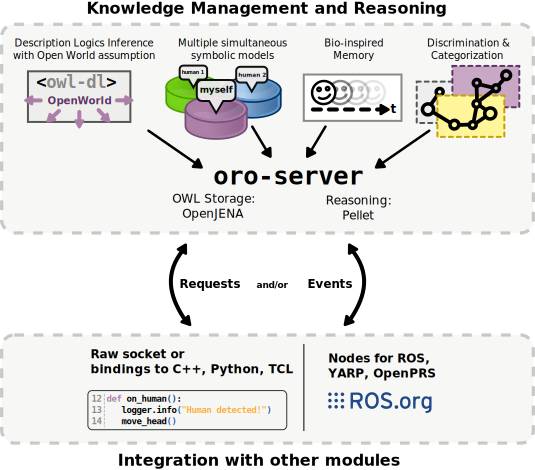
\includegraphics[width=0.75\columnwidth]{oroserver/oro_architecture_functional.pdf}
  \caption{Overview of the ORO architecture.}
  \label{fig|oro-overview}
\end{figure}

At the core, ORO is build around the
OpenJena\footnote{\url{http://www.openjena.org}} ontology management library,
connected to the Pellet\footnote{\url{http://clarkparsia.com/pellet}}
reasoner.

A front-end accepts and manages connections to clients. The clients' requests
are processed by a set of internal modules: basic operations on statements, but
also higher cognitive and human-robot interaction related features are
available. External plugins can also be added via a specific extension
mechanism.

Besides acting as a facts database, the ORO platform exposes several
functions: operations on knowledge statements relying on inference (through a
continuous first-order logic classification process), management of
\emph{per-agent} symbolic models, categorisation of sets of concepts
and profiles of memory (that enable the robot to ``forget'' about some facts).

ORO also provides an event mechanism that allows components to be triggered
when specific events occur. A component can for instance subscribe to events
of kind \setstmt{?agent isVisible true, ?agent type Human}. As soon as the
perception layer detects a human in the robot's field of view and accordingly
updates the knowledge base, the executive layer is triggered. The event
framework also takes advantage of the inference capabilities of ORO. Thus an
event can be indirectly triggered if its triggering conditions can be
inferred to be true.

\subsubsection{Representation of alternative knowledge models}
\label{sect|alterite}

As pictured in Figure~\ref{fig|oro-overview}, ORO stores independent cognitive
models for each agent it interacts with. When the ORO server actually
identifies a new agent (or infers that some instance is an agent), it
automatically creates a new, separate, in-memory OWL model for that agent.
Then, different robot components, like execution control or situation
assessment, may store the agents' beliefs in separate, independent models. All
knowledge processing functions in the robot's primary model are equally
available in every agent's model, which allows us to store and reason on
different (and possibly globally inconsistent) models of the world.

Each of these models is independent and logically consistent, enabling
reasoning on different perspectives of the world that would otherwise be
considered as globally inconsistent (for instance, an object can be visible for
the robot but not for the human. This object can have at the same time the
property \concept{isVisible \textit{true}} and \concept{isVisible
\textit{false}} in two different models).

We present at section~\ref{sect|spark}, page~\pageref{sect|spark}, a 3D
real-time environment, SPARK, that allows to compute on-line several symbolic
properties that are dependent on the perspectives.

\paragraph{Theory Of Mind and contexts} \label{sect|theory-of-mind}

By maintaining independent mental states for each agent it interacts with, we
consider the robot to be endowed with a simple \emph{theory of
mind}~\cite{Scassellati2002}: the robot can explicitly model the beliefs of its
interactors, it expose them to the control architecture, and the same set of
cognitive abilities are available on these secondary model as on the main
model: reasoning, inconsistencies detection, events, etc.

Proper \emph{false beliefs} experiment, similar to the Sally and Ann experiment
presented in the previous chapter, has been recently conducted with ORO
by Mathieu Warnier, as reported in~\cite{Warnier2012a}: in this experiment, two
humans observe a table with several objects, then one leaves while the other
one moves around some objects. This leads to two different set of beliefs on
the world, which the robot explicitly stores and updates when necessary (if the
human comes back and check the table, for instance).

These multiple models can also be viewed as different \emph{interpretive
frames}, allowing the robot to interpret the same reality from different points
of view. In this sense, each model carries a context of interaction.  In
chapter~\ref{chapt|dialogs}, we present how such agent-dependent contexts are
used by a natural language processor to make sense of user sentences from
his/her point of view.

\subsection{Reasoning techniques}

\subsubsection{Standard inference services}
\subsubsection{Grounding, classification and discrimination algorithms}
\subsubsection{Memory}
\subsubsection{Knowledge structure alteration and learning}



\section{Knowledge instantiation: the OpenRobots Common-Sense Ontology}
\label{sect|oro-commonsense}

The ORO platform is made of the server that we have presented, and a
common-sense ontology, the \emph{ORO Common-sense Ontology}.

At start-up, the knowledge model of the ORO server is initialised with a
configurable sets of ontologies that build together the initial pool of facts
known to the robot: the common-sense ontology and optional, domain dependent
ontologies.

Each time a new model is created (typically when a new agent is detected), it
is also initialised with the same pool of facts.  From the point of view of the
robot, this ensure that all the different agents share the same background
knowledge.

Usually, the ORO server is started with the common-sense ontology that we
present in this section, and one scenario-specific ontology that usually
contains the set of individuals with relevant properties needed by the
experiment.

\begin{figure}
    \centering
    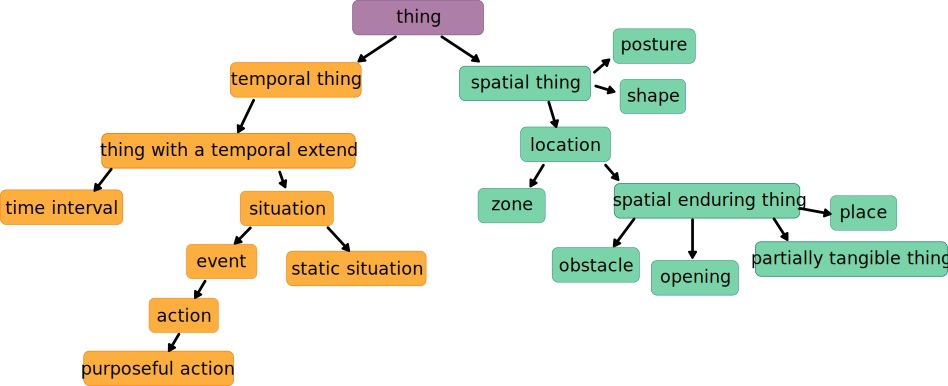
\includegraphics[scale=0.6]{oro/top_tbox.pdf}

    \caption{The upper part of the ORO common-sense TBox. All these concepts
    belong to the {\sc OpenCyc} namespace.}
    
    \label{fig|upper_tbox}
\end{figure}

The ORO common-sense ontology has been designed from two requirements: covering
our experimental needs and conforming as much as possible to the {\sc OpenCyc}
upper ontology.

This lead to a bidirectional design process: from \emph{bottom-up} regarding
the choices of concepts to model, \emph{top-down} regarding the upper part of the
taxonomy. This upper part of the ontology is pictured on
figure~\ref{fig|upper_tbox}. All the classes visible on this figure belong to the
{\sc OpenCyc} namespace (the {\tt cyc:} prefix is omitted).

This figure~\ref{fig|upper_tbox} also illustrates the fundamental disjunction
in the ORO model between \emph{temporal} and \emph{spatial} entities (formally,
$(TemporalThing \sqcap SpatialThing)^{\mathcal{I}} = \emptyset$, with
$\mathcal{I}$ the \emph{interpretation} of our model).

The class \concept{purposeful action} is the superset of all the actions that
are voluntarily performed by the robot (or another agent). Subclasses (like
\concept{Give}, \concept{LookAt}, etc.) are not asserted in the common-sense
ontology, but are added by the execution controller (in link with the symbolic
task planner) and the natural language processor based on what is actually
performable and/or understandable by the robot at run-time.

...mention thqt other pqrts like objects qre much more refined.

Lastly, the ORO common-sense ontology contains several rules and class
expressions that encode non-trivial inferences.

The definition of the \concept{Bottle} is a case in point. We already gave a
simplified version, here the complete definition:

\concept{Bottle} $\equiv$ \concept{Container} {\bf and} \concept{Tableware}
{\bf that} (\concept{hasShape} {\bf value} \concept{cylinderShape} {\bf and}
\concept{hasCharacteristicDimension} {\bf only} \concept{\em int[>= 0.1, <=
0.3]})

If a human informs the robot that a given object is indeed a bottle, the robot
can then infer much more on this object. And if the human affirms that a car is
a bottle, the robot may question this assertion because of the inconsistent
size.

%%%%%%%%%%%%%%%%%%%%%%%%%%%%%%%%%%%%%%%%%%%%%%%%%%%%%%%%%%%%%%%%%%%%%%%%%%%%%%%
%%%%%%%%%%%%%%%%%%%%%%%%%%%%%%%%%%%%%%%%%%%%%%%%%%%%%%%%%%%%%%%%%%%%%%%%%%%%%%%
%%%%%%%%%%%%%%%%%%%%%%%%%%%%%%%%%%%%%%%%%%%%%%%%%%%%%%%%%%%%%%%%%%%%%%%%%%%%%%%
\section{Integration in the robot architecture}
\label{sect|integration}

\begin{figure*}[thpb]
  \centering
  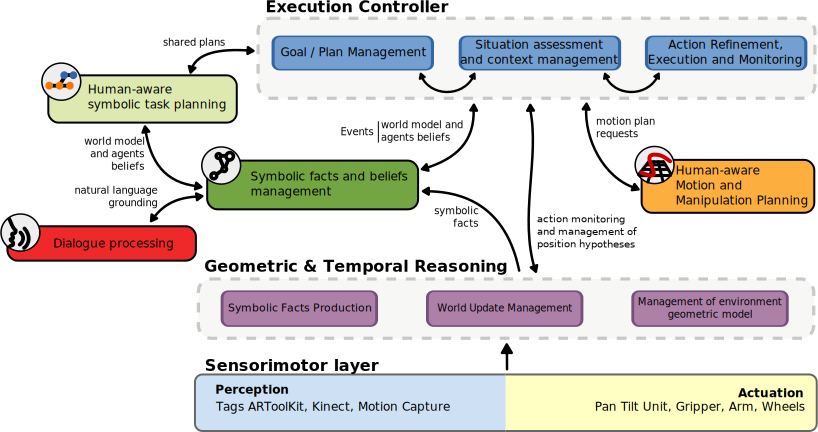
\includegraphics[width=\columnwidth]{integration/architecture_overview.pdf}

  \caption {Software architecture of PR2 and Jido, two service robot
  interacting with humans at LAAS-CNRS.}

  \label{fig|archi}
\end{figure*}

Figure~\ref{fig|archi} presents the organisation of the upper software layer
(the ``decisional'' or ``cognitive'' layer) of the service robots Jido and PR2
as currently in service at LAAS (this architecture is described in detail
in~\cite{Alami2011}). The sensori-motor layer (bottom) is abstracted in SPARK,
an intermediate amodal 3D model where geometric (and some temporal) reasoning
take place.

The outcome of the geometric analysis, as well as the result of the dialogue
processing module ({\sc Dialogs}), are stored in ORO, that plays the role of as
a central knowledge hub. The symbolic knowledge base triggers events that are
captured by a top-level execution controller.

In our architecture, the controller can rely on two specialised planners: MHP,
a geometric motion and manipulation planner~\cite{Sisbot2008, Mainprice2011,
Pandey2010} and HATP, a symbolic task planner~\cite{Alili2009}.

The dialogue processing module, as well as the symbolic task planner, also use
the knowledge base to answer questions or initialise the planning domain.

During a typical interaction experiment (such an experiment is describe at
chapter~\ref{chapt|evaluation}), the execution controller decides upon a goal
to reach, requires a plan from the task planner, allocates the actions to the
human and the robot, communicates the shared plan to the human, and controls
and monitors its execution. The operation continues until the goal is achieved,
is declared unachievable or is abandoned by the human.

In this architecture, only ORO and Dialogs (the dialogue processing module that
we present in the next chapter), as components, are the actual direct outcomes
of this doctoral work. It is however important to present the other one all
here as well since a knowledge base only make sense within a larger
architecture, with knowledge providers and consumers.  Furthermore, the
approach to knowledge management introduced by this thesis had a strong
influence on the design of the communication flows between all these
components. Thus, this section introduces the software components that have
been used in conjunction with ORO (mostly, but not only, on the LAAS robots),
and details how these components produce, exchange and consume symbolic
knowledge.


